\chapter{Getting Started with Path Tracing: Tutorial}\labappendix{tutorial}

This appendix provides a step-by-step tutorial on performing (differentiable) path tracing based on the advanced path tracing tutorial available in the documentation of the DiffeRT Python library~\sidecite{Eertmans2025ICMLCNDemo}. It explores the library's lower-level \gls{api} and the underlying logic used to perform exact path tracing. We first focus on the image method in a simple scene, then illustrate scaling limits and pruning mechanisms in larger environments, and finally present ray launching as an alternative strategy. Notation and terminology follow \refch{path-tracing} and \refch{efficient-path-tracing}. The differentiability aspects of the implementation are not covered here, as they are automatically handled by the library's use of JAX as the underlying computational framework. For more details on the differentiable components, readers are encouraged to consult the library's documentation and source code.

\section{Example on a Simple Scene}
\label{sec:tutorial_simple_scene}

Before diving into a complex scene, it is helpful to use a very simple setup to understand the fundamental steps of path tracing.

Note that the high-level \texttt{TriangleScene.compute\_paths} method implicitly handles all the logic presented in this section, as well as the optimizations and post-processing steps omitted here for clarity.

\subsection{Scene Loading and Setup}
\label{sec:rt_step1}

The first step is to define the propagation environment. In modern ray tracers, this is typically done by loading a mesh file (e.g., \texttt{.obj} or \texttt{.ply}) that represents the physical geometry, such as buildings or terrain. \reflisting{differt-loading-scene} shows how to load a simple scene with two buildings and define the transmitter and receiver positions. The mesh is loaded into a \texttt{TriangleMesh} structure, which contains vertices and face indices:

\begin{enumerate}
  \item This structure can also define sub-meshes to group primitives (e.g., walls and ground), radio materials, and face colors.
  \item The positions of the transmitter ($\bsup{x}_\text{\glsxtrshort{tx}}$) and receiver ($\bsup{x}_\text{\glsxtrshort{rx}}$) are defined as coordinates in $\mathbb{R}^3$. The antenna properties are not relevant for path tracing, so they are not considered here.
\end{enumerate}

\begin{listing}
  \caption{Loading a simple scene in DiffeRT.}
  \lablisting{differt-loading-scene}
  \inputmintedmarker[]{python}{codes/wide/tutorial.py}{scene_loading}
\end{listing}

\begin{figure}
  \centering
  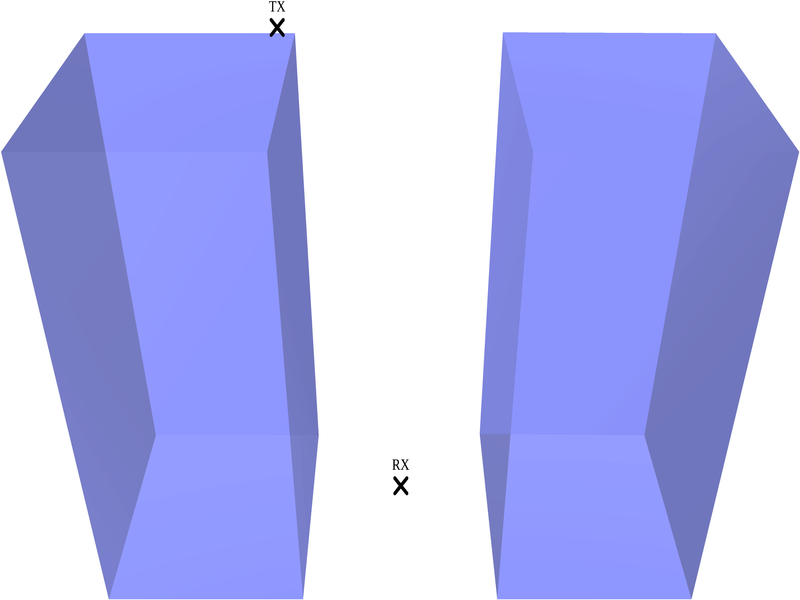
\includegraphics[width=\textwidth]{images/tutorial-simple-scene.png}
  \caption{Simple scene with two buildings, a \glsxtrshort{tx}, and an \glsxtrshort{rx}.}
  \labfig{tutorial-simple-scene}
\end{figure}

For more advanced scenarios, DiffeRT also supports loading scenes from the Mitsuba3 XML~\sidecite[-3\baselineskip]{Jakob2022Mitsuba3} format, as used by Sionna~RT~\sidecite[-2\baselineskip]{Hoydis2023}.

\subsection{How We Trace Rays: The Graph Analogy}

Ray tracing can be implemented in many ways, depending on the desired performance, required accuracy, and geometry representation. Here, we implement exhaustive (or \textit{exact}) ray tracing by generating all possible paths from \glsxtrshort{tx} to \glsxtrshort{rx} that undergo up to a maximum number of interactions (e.g., reflections) with the environment.

As first discussed in \refch{path-tracing}, one way to frame this is to represent the problem as a graph. The goal is to find paths from the \glsxtrshort{tx} node to the \glsxtrshort{rx} node, possibly visiting intermediate nodes corresponding to specific primitives (triangles) in the scene. A graph algorithm thus generates a list of path candidates. A candidate is not a physical path with 3D coordinates, but rather an ordered list of interactions to visit. A deeper discussion of how to generate candidates is provided in \refappendix{path_candidates}.

It is then the role of a path tracing method (e.g., the image method) to determine the exact coordinates of that path. For the formal definition of path candidates and exact-coordinate recovery, see \refch{path-tracing}.

\subsection{Solving for Path Vertices using the Image Method}

For each generated path candidate, we must calculate the exact coordinates of the reflection points. The mathematical derivation of the image method (forward image construction and backward intersection pass) is detailed in \refch{path-tracing}; here we only show the corresponding implementation.

If we manually select a subset of triangles (e.g., from the red surface and the green surface), we can trace paths of increasing order (e.g., \glsxtrshort{tx} $\to$ \glsxtrshort{rx}, \glsxtrshort{tx} $\to$ red $\to$ \glsxtrshort{rx}, \glsxtrshort{tx} $\to$ red $\to$ green $\to$ \glsxtrshort{rx}).

\begin{listing*}
  \caption{Manual path tracing with the image method for orders 0, 1, and 2.}
  \lablisting{differt-manual-image-method}
  \inputmintedmarker[]{python}{codes/wide/tutorial.py}{manual_image_method}
\end{listing*}

\begin{figure}
  \centering
  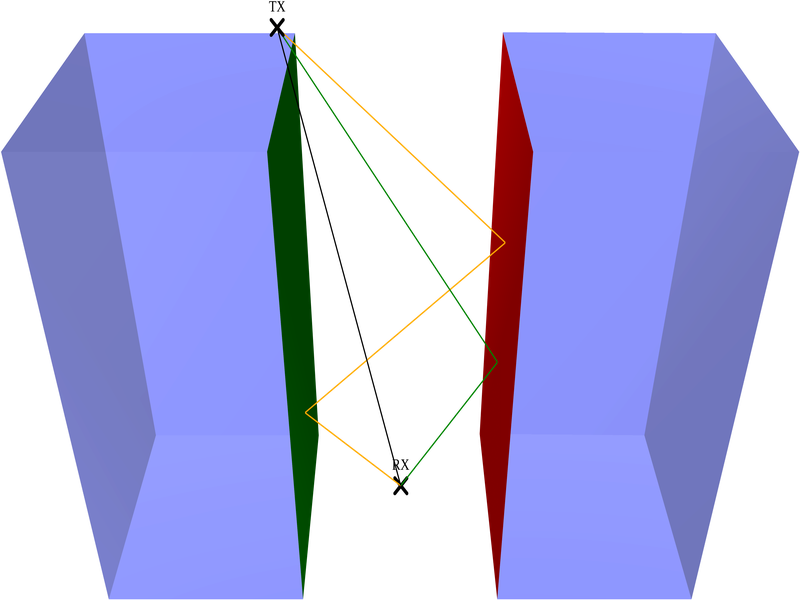
\includegraphics[width=\textwidth]{images/tutorial-image-method-orders-0-2.png}
  \caption{Paths traced with the Image Method for order 0 (\gls{line-of-sight}), order 1, and order 2.}
  \labfig{tutorial-image-method-orders}
\end{figure}

\subsection{Generating All Path Candidates}

Manually identifying surfaces and generating all possible path candidates rapidly becomes tedious as the number of surfaces or the path order increases. For this purpose, DiffeRT provides \texttt{generate\_all\_path\_candidates}. Written in Rust for performance, this function can generate millions of path candidates per second for a fixed maximum reflection order $K$. See \refsec{computational-complexity} for a complexity discussion and \refsec{exponential-path-generation} for the image-tree perspective. In the simplified case of specular reflections, a path candidate can be formally defined as a sequence of triangle (also referred to as primitive) indices
\begin{equation}
  \bsup{I} = \left[p_1, p_2, \ldots, p_k, \ldots, p_K\right],
\end{equation}
where $K$ is the path order (number of interactions) and $p_k$ is the index of the primitive involved in the $k$-th interaction. The aforementioned function generates all possible combinations of primitives for a fixed path order, excluding path candidates with two consecutive identical primitives (as reflecting twice off the same flat surface is not possible), resulting in a comprehensive list of path candidates that can be further processed to determine their validity and physical parameters.

For more details on generating candidates, refer to \refappendix{path_candidates}.

\subsection{Path Validation}

Generating all possible candidates has one major side effect that we already discussed: many paths will be invalid (e.g., they might pass through a building or miss the mirror entirely). Furthermore, because the image method assumes infinite planes for its calculations, we must validate our paths against a series of geometric checks, consistent with \refsec{combinatorial-bottleneck}.

After computing the exact coordinates of the reflection points for each candidate, we apply a series of checks to filter out invalid paths:
\begin{enumerate}
  \item A \emph{finite triangle check} verifies that each computed reflection point lies within the boundaries of its corresponding finite triangle.
  \item An \emph{interaction order check} ensures that all interactions respect the physical laws of reflection (e.g., incident and reflected rays must hit the same side of the mirror).
  \item An \emph{occlusion check (ray--triangle intersection)} detects \gls{line-of-sight} obstructions. Even if a reflection point is valid, the ray traversing the scene must not be blocked by any other object.
\end{enumerate}

\begin{listing*}
  \ContinuedFloat*
  \caption{All ray tracing steps assembled: candidate generation, geometry inputs, and path computation.}
  \inputmintedmarker[]{python}{codes/wide/tutorial.py}{image_method_all_orders_a}
\end{listing*}

\begin{listing*}
  \ContinuedFloat
  \caption{All ray tracing steps assembled (continued): first validity check.}
  \inputmintedmarker[]{python}{codes/wide/tutorial.py}{image_method_all_orders_b}
\end{listing*}

\begin{listing*}
  \ContinuedFloat
  \caption{All ray tracing steps assembled (continued): occlusion filtering and final path extraction.}
  \inputmintedmarker[]{python}{codes/wide/tutorial.py}{image_method_all_orders_c}
\end{listing*}

\begin{figure*}
  \centering
  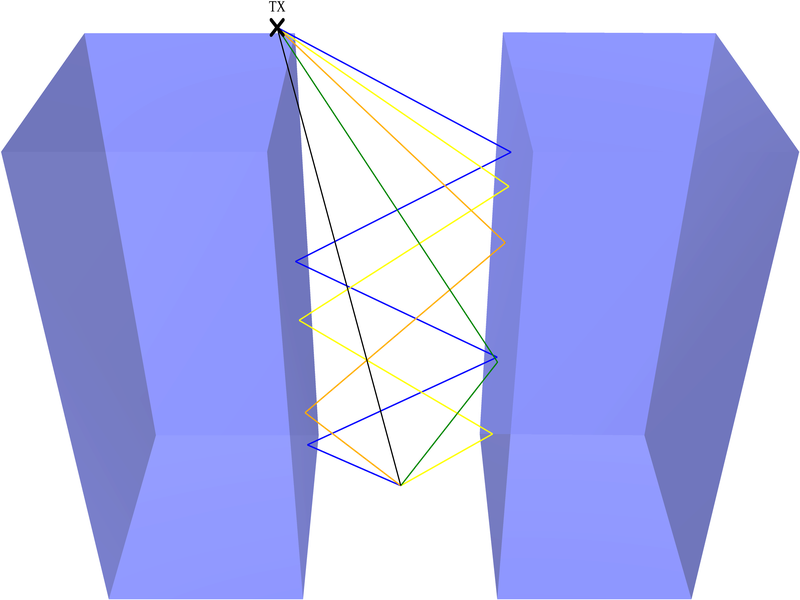
\includegraphics[width=\textwidth]{images/tutorial-all-orders-valid-paths.png}
  \caption{Validated paths after applying boundary, interaction-side, and occlusion checks.}
  \labfig{tutorial-all-orders-valid-paths}
\end{figure*}

As mentioned earlier, running this manually is cumbersome. However, we can accomplish all of this with a single call to \texttt{TriangleScene.compute\_paths}, as shown in \reflisting{differt-compute-paths}.

\begin{listing}
  \caption{Computing ray paths with the high-level \gls{api}.}
  \lablisting{differt-compute-paths}
  \inputminted[firstline=1,lastline=8]{python}{codes/differt-compute-paths.py}
\end{listing}

\section{Scaling to Complex Scenes}

While exact path tracing works gracefully on simple scenes, it scales poorly to environments with millions of primitives---like modern city models.

\subsection{The Combinatorial Explosion}

The function \texttt{generate\_all\_path\_candidates} returns an array of size $N_{\text{triangles}} \times (N_{\text{triangles}}-1)^{\text{order}-1} \times \text{order}$, leading directly to the combinatorial bottleneck previously discussed in \refch{efficient-path-tracing}. For instance, a modestly sized city scene can quickly generate hundreds of millions of second-order paths that require evaluation.

For large scenes, the size of the candidate array quickly exceeds the available memory. To address this issue, DiffeRT offers an iterator variant called \texttt{generate\_all\_path\_candidates\_chunks\_iter} that yields smaller arrays in chunks. While this solves the memory exhaustion issue, it does not reduce the massive computational load of tracing and checking these paths. Therefore, we must attempt to reduce the number of path candidates \emph{before} generating them.

\begin{figure}
  \centering
  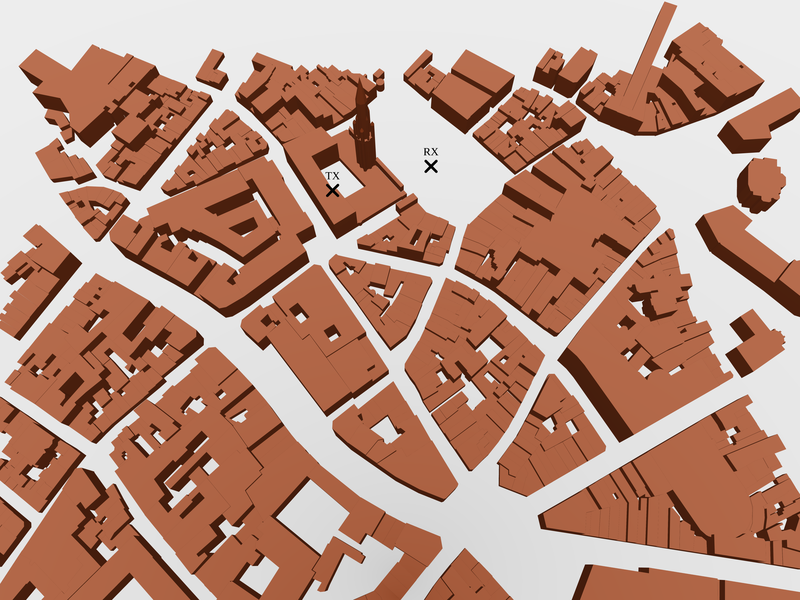
\includegraphics[width=\textwidth]{images/tutorial-complex-scene-setup.png}
  \caption{Large urban scene---Grand Place of Brussels---used to illustrate combinatorial growth and pruning strategies.}
  \labfig{tutorial-complex-scene-setup}
\end{figure}

\subsection{Assuming Quadrilaterals}

In many cases, architectural scenes primarily consist of quadrilaterals that have been trivially split into two triangles. Configuring the library to assume quadrilaterals via \texttt{mesh.set\_assume\_quads(True)} effectively halves the number of individual primitives. Since the number of candidates scales with $N_{\text{triangles}} \times (N_{\text{triangles}}-1)^{\text{order}-1}$, halving the primitives reduces the total candidates by nearly a factor of $2^{\text{order}}$.

A summary of the number of path candidates for second-order reflection paths and the effect of assuming quadrilaterals is provided below for the large urban scene shown in \reffig{tutorial-complex-scene-setup}.
\begin{minted}{text}
# Number of primitives (triangles): 14 206
# Number of path candidates: 201 796 230
# Number of primitives (assume_quads=True): 7 103
# Number of path candidates: 50 445 506
\end{minted}

\subsection{Determining Transmitter Visibility for Graph Pruning}

A highly effective way to prune path candidates is to recognize that the transmitter (or receiver) cannot physically reach all objects in the scene. By assessing which triangles are visible from \glsxtrshort{tx} using \texttt{triangles\_visible\_from\_vertices}, we can construct a visibility vector, shrinking the pool of potential target nodes in the graph. This corresponds to the visibility preprocessing strategy of \refch{efficient-path-tracing}.

\begin{listing*}
  \caption{Estimating triangle visibility from \glsxtrshort{tx} and recoloring the mesh.}
  \lablisting{differt-visibility-from-tx}
  \inputmintedmarker[]{python}{codes/wide/tutorial.py}{visibility_from_tx}
\end{listing*}

\begin{figure}
  \centering
  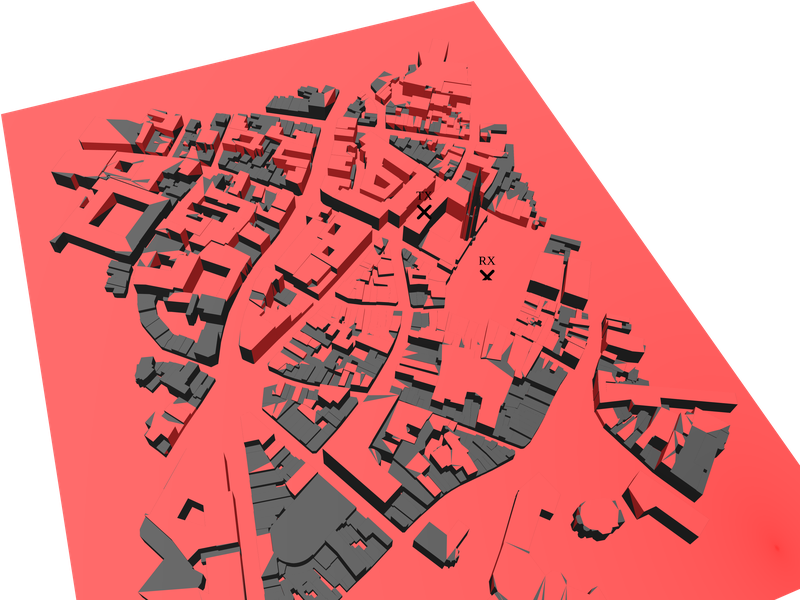
\includegraphics[width=\textwidth]{images/tutorial-visibility-from-tx.png}
  \caption{Triangles visible from \glsxtrshort{tx} (red) versus hidden triangles (dark) for the large scene.}
  \labfig{tutorial-visibility-from-tx}
\end{figure}

The percentage of visible triangles can be quite low in dense urban scenes, leading to a dramatic reduction in path candidates. Example numbers for the large urban scene are provided below.
\begin{minted}{text}
# Percentage of visible triangles: 17.72%
# Percentage of visible quadrilaterals: 26.81%
# Number of path candidates: 13 522 208
\end{minted}

Moreover, if the geometry is static, we can precompute the visibility vector of \textit{every} triangle to every other triangle, constructing a massive adjacency (visibility) matrix. Instead of using a \texttt{CompleteGraph}, this matrix allows us to instantiate a \texttt{DiGraph} representation (see \refappendix{path_candidates} for more details). By explicitly disconnecting mutually invisible primitives within the topological graph, we dramatically prune the theoretical path candidates, preventing wasted computations on segments that are physically obstructed. However, this approach becomes infeasible for very large scenes due to the quadratic growth of the adjacency matrix size with the number of primitives, and because the precomputed visibility, which relies on ray casting, may not be exact.

\section{An Alternative: Ray Launching}

Eventually, any exact method, even heavily pruned, encounters a practical limit. Highly dense scenes or requests for high-order interactions will cause the sheer number of path candidates to overwhelm optimizations. In these scenarios, ray launching methods, such as \gls{sbr}, serve as a viable alternative (see also the inexact methods overview in \refch{path-tracing}).

Unlike exact graph-based methods, \gls{sbr} launches a fixed, manageable number of mathematical rays radially outward from \glsxtrshort{tx}. These rays traverse the environment and undergo a constrained number of reflections off consecutive surfaces. Before each reflection event, the trajectory is scanned to determine whether it passes within an acceptable radius of the receiver (\glsxtrshort{rx}). If so, the sequence of reflections is harvested and implicitly formulated as a path, often followed by a localized final \enquote{correction} to align the endpoint strictly with \glsxtrshort{rx}. To avoid casting rays in directions that are unlikely to yield valid paths, launching can be guided by a coarse visibility analysis or by importance sampling based on the antenna pattern. Here, the rays are launched within the boundaries of the scene, as determined by the viewing frustum of the transmitter. \reflisting{differt-sbr} shows a simplified implementation. For efficient looping, the implementation relies on JAX's \texttt{jax.lax.scan} function.

\begin{listing*}
  \ContinuedFloat*
  \caption{Simplified \gls{sbr} implementation: setup and ray launch parameters.}
  \lablisting{differt-sbr}
  \inputmintedmarker[]{python}{codes/wide/tutorial.py}{sbr_a}
\end{listing*}

\begin{listing*}
  \ContinuedFloat
  \caption{Simplified \gls{sbr} implementation (continued): computing the next bounce (scan function).}
  \inputmintedmarker[]{python}{codes/wide/tutorial.py}{sbr_b}
\end{listing*}

\begin{listing*}
  \ContinuedFloat
  \caption{Simplified \gls{sbr} implementation (continued): detecting intersections with reception sphere (scan function).}
  \inputmintedmarker[]{python}{codes/wide/tutorial.py}{sbr_c}
\end{listing*}

\begin{listing*}
  \ContinuedFloat
  \caption{Simplified \gls{sbr} implementation (continued): reflecting rays (scan function).}
  \inputmintedmarker[]{python}{codes/wide/tutorial.py}{sbr_d}
\end{listing*}

\begin{listing*}
  \ContinuedFloat
  \caption{Simplified \gls{sbr} implementation (continued): scan execution and path assembly.}
  \inputmintedmarker[]{python}{codes/wide/tutorial.py}{sbr_e}
\end{listing*}

\begin{figure*}
  \centering
  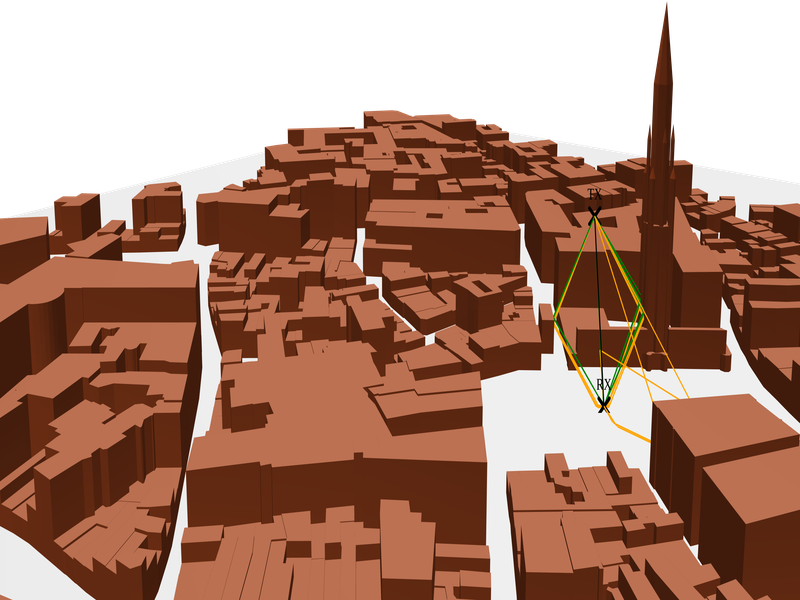
\includegraphics[width=\contentwidth]{images/tutorial-sbr-paths.png}
  \caption{Up to second-order reflection paths found with the \gls{sbr} method that pass near \glsxtrshort{rx} in the large urban scene. Note that the double-counting problem is not addressed here, and duplicate paths are not removed.}
  \labfig{tutorial-sbr-paths}
\end{figure*}

Because path candidates are never explicitly generated beforehand, \gls{sbr} smoothly bypasses the combinatorial explosion. The computational cost roughly scales with the chosen resolution of launched rays instead of strictly with the mesh fidelity. Within DiffeRT, this behavior can be natively invoked by providing \texttt{method='sbr'} when calling \texttt{TriangleScene.compute\_paths}.

\section{Summary}

This tutorial demonstrates, in executable form, the workflow discussed in \refch{path-tracing} and \refch{efficient-path-tracing}: candidate generation, exact-coordinate recovery, validation, pruning, and an inexact alternative via \gls{sbr}. Ultimately, the DiffeRT pipeline abstracts these low-level routines to produce validated geometric trajectories, which parameterize the computation of channel impulse responses, delays, and signal power. For further insight and fully reproducible notebooks, readers are invited to consult the library's online documentation.
